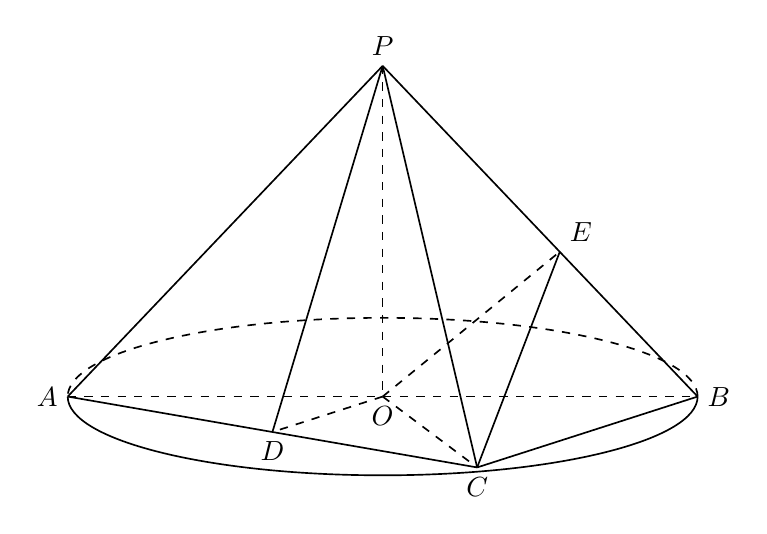
\begin{tikzpicture}[x=1cm,y=1cm,line width=0.6pt]
\coordinate (O) at (0,0);
\coordinate (A) at (-4,0);
\coordinate (B) at (4,0);
\coordinate (P) at (0,4.2);
\coordinate (C) at (1.2,-0.9);
\coordinate (D) at (-1.4,-0.45);
\coordinate (E) at (2.25,1.84);
% base circle: back dashed, front solid
\draw[dashed] (B) arc (0:180:4 and 1);
\draw (A) arc (180:360:4 and 1);
% diameter (hidden, drawn over front arc for clarity as dashed)
\draw[dashed] (A) -- (B);
% axis
\draw[dashed] (P) -- (O);
% lateral generators
\draw (P) -- (A);
\draw (P) -- (B);
\draw (P) -- (D);
\draw (P) -- (C);
% base chords
\draw (A) -- (D) -- (C);
\draw (B) -- (C);
\draw (E) -- (C);
% hidden segments from centre
\draw[dashed] (O) -- (D);
\draw[dashed] (O) -- (C);
\draw[dashed] (O) -- (E);
% labels
\node[above] at (P) {$P$};
\node[left] at (A) {$A$};
\node[right] at (B) {$B$};
\node[below] at (O) {$O$};
\node[below] at (D) {$D$};
\node[below] at (C) {$C$};
\node[above right] at (E) {$E$};
\end{tikzpicture}
